%%%%%%%%%%%%%%%%%%%%%%%%%%%%%%%%%%%%%%%%%
% Programming/Coding Assignment
% LaTeX Template
%
% This template has been downloaded from:
% http://www.latextemplates.com
%
% Original author:
% Ted Pavlic (http://www.tedpavlic.com)
% Minor package modifications made by Robert Balayan
%
% Note:
% The \lipsum[#] commands throughout this template generate dummy text
% to fill the template out. These commands should all be removed when
% writing assignment content.
%
% This template uses a Perl script as an example snippet of code, most other
% languages are also usable. Configure them in the "CODE INCLUSION
% CONFIGURATION" section.
%
%%%%%%%%%%%%%%%%%%%%%%%%%%%%%%%%%%%%%%%%%

%----------------------------------------------------------------------------------------
%	PACKAGES AND OTHER DOCUMENT CONFIGURATIONS
%----------------------------------------------------------------------------------------




\documentclass{article}

\usepackage{fancyhdr} % Required for custom headers
\usepackage{lastpage} % Required to determine the last page for the footer
\usepackage{extramarks} % Required for headers and footers
\usepackage[usenames,dvipsnames]{color} % Required for custom colors
\usepackage{graphicx} % Required to insert images
\usepackage{subcaption}
\usepackage{enumitem}
\usepackage{listings} % Required for insertion of code
\usepackage{courier} % Required for the courier font
\usepackage{lipsum} % Used for inserting dummy 'Lorem ipsum' text into the template
\usepackage{pgf}
\usepackage{dcolumn}
\usepackage{booktabs}
\usepackage{tikz}
\usetikzlibrary{arrows,automata}
\usetikzlibrary{positioning,shapes,arrows}
\newcolumntype{M}[1]{D{.}{.}{1.#1}}
\usepackage[utf8]{inputenc}
\usepackage{amsfonts}
\usepackage{amsmath}
\usepackage{amsthm}
\usepackage{cite}
\usepackage{hyperref}
\hypersetup{
    colorlinks=true,
    linkcolor=blue,
    filecolor=magenta,
    urlcolor=blue,
}
\usepackage{wrapfig}
\usepackage{algorithm}
\usepackage{algpseudocode}
\algnewcommand\algorithmicinput{\textbf{Input:}}
\algnewcommand\algorithmicoutput{\textbf{Output:}}
\algnewcommand\Input{\item[\algorithmicinput]}
\algnewcommand\Output{\item[\algorithmicoutput]}
\renewcommand{\algorithmicforall}{\textbf{foreach}}


% Margins
\topmargin=-0.45in
\evensidemargin=0in
\oddsidemargin=0in
\textwidth=6.5in
\textheight=9.0in
\headsep=0.25in

\linespread{1.2} % Line spacing

% Some useful macros.
\newcommand{\given}{\,|\,}
\newcommand{\R}{\mathbb{R}}
\newcommand{\E}{\mathbb{E}}
\newcommand{\var}{\text{var}}
\newcommand{\cov}{\text{cov}}
\newcommand{\trans}{\mathsf{T}}
\newcommand{\bx}{\mathbf{x}}
\newcommand{\by}{\mathbf{y}}
\newcommand{\bw}{\mathbf{w}}
\newcommand{\distNorm}{\mathcal{N}}
\newcommand{\bzero}{\mathbf{0}}
\newcommand{\btheta}{\boldsymbol{\theta}}
\newcommand{\bpi}{\boldsymbol{\pi}}
\newcommand{\ident}{\mathbb{I}}
\newcommand{\N}{\mathcal{N}}
\newcommand{\ep}{\varepsilon}
\newcommand{\Dir}{\text{Dirichlet}}

% Set up the header and footer
\pagestyle{fancy}
\lhead{\hmwkAuthorName} % Top left header
\rhead{\hmwkTitle} % Top center head
%\rhead{\firstxmark} % Top right header
\cfoot{} % Bottom center footer
\rfoot{Page\ \thepage\ of\ \protect\pageref{LastPage}} % Bottom right footer
\renewcommand\headrulewidth{0.4pt} % Size of the header rule
\renewcommand\footrulewidth{0.4pt} % Size of the footer rule

%\setlength\parindent{0pt} % Removes all indentation from paragraphs

%----------------------------------------------------------------------------------------
%	CODE INCLUSION CONFIGURATION
%----------------------------------------------------------------------------------------

\definecolor{MyDarkGreen}{rgb}{0.0,0.4,0.0} % This is the color used for comments
\lstloadlanguages{Perl} % Load Perl syntax for listings, for a list of other languages supported see: ftp://ftp.tex.ac.uk/tex-archive/macros/latex/contrib/listings/listings.pdf
\lstset{language=Perl, % Use Perl in this example
        frame=single, % Single frame around code
        basicstyle=\small\ttfamily, % Use small true type font
        keywordstyle=[1]\color{Blue}\bf, % Perl functions bold and blue
        keywordstyle=[2]\color{Purple}, % Perl function arguments purple
        keywordstyle=[3]\color{Blue}\underbar, % Custom functions underlined and blue
        identifierstyle=, % Nothing special about identifiers
        commentstyle=\usefont{T1}{pcr}{m}{sl}\color{MyDarkGreen}\small, % Comments small dark green courier font
        stringstyle=\color{Purple}, % Strings are purple
        showstringspaces=false, % Don't put marks in string spaces
        tabsize=5, % 5 spaces per tab
        %
        % Put standard Perl functions not included in the default language here
        morekeywords={rand},
        %
        % Put Perl function parameters here
        morekeywords=[2]{on, off, interp},
        %
        % Put user defined functions here
        morekeywords=[3]{test},
       	%
        morecomment=[l][\color{Blue}]{...}, % Line continuation (...) like blue comment
        numbers=left, % Line numbers on left
        firstnumber=1, % Line numbers start with line 1
        numberstyle=\tiny\color{Blue}, % Line numbers are blue and small
        stepnumber=5 % Line numbers go in steps of 5
}

% Creates a new command to include a perl script, the first parameter is the filename of the script (without .pl), the second parameter is the caption
\newcommand{\perlscript}[2]{
\begin{itemize}
\item[]\lstinputlisting[caption=#2,label=#1]{#1.pl}
\end{itemize}
}

%----------------------------------------------------------------------------------------
%	DOCUMENT STRUCTURE COMMANDS
%	Skip this unless you know what you're doing
%----------------------------------------------------------------------------------------

% Header and footer for when a page split occurs within a problem environment
\newcommand{\enterProblemHeader}[1]{
%\nobreak\extramarks{#1}{#1 continued on next page\ldots}\nobreak
%\nobreak\extramarks{#1 (continued)}{#1 continued on next page\ldots}\nobreak
}

% Header and footer for when a page split occurs between problem environments
\newcommand{\exitProblemHeader}[1]{
%\nobreak\extramarks{#1 (continued)}{#1 continued on next page\ldots}\nobreak
%\nobreak\extramarks{#1}{}\nobreak
}

%\setcounter{secnumdepth}{0} % Removes default section numbers
%\newcounter{homeworkProblemCounter} % Creates a counter to keep track of the number of problems
%\setcounter{homeworkProblemCounter}{-1}

\newcommand{\homeworkProblemName}{}
\newenvironment{homeworkProblem}[1][Problem \arabic{homeworkProblemCounter}]{ % Makes a new environment called homeworkProblem which takes 1 argument (custom name) but the default is "Problem #"
\stepcounter{homeworkProblemCounter} % Increase counter for number of problems
\renewcommand{\homeworkProblemName}{#1} % Assign \homeworkProblemName the name of the problem
\section{\homeworkProblemName} % Make a section in the document with the custom problem count
\enterProblemHeader{\homeworkProblemName} % Header and footer within the environment
}{
\exitProblemHeader{\homeworkProblemName} % Header and footer after the environment
}

\newcommand{\problemAnswer}[1]{ % Defines the problem answer command with the content as the only argument
\noindent\framebox[\columnwidth][c]{\begin{minipage}{0.98\columnwidth}#1\end{minipage}} % Makes the box around the problem answer and puts the content inside
}

\newcommand{\homeworkSectionName}{}
\newenvironment{homeworkSection}[1]{ % New environment for sections within homework problems, takes 1 argument - the name of the section
\renewcommand{\homeworkSectionName}{#1} % Assign \homeworkSectionName to the name of the section from the environment argument
\subsection{\homeworkSectionName} % Make a subsection with the custom name of the subsection
\enterProblemHeader{\homeworkProblemName\ [\homeworkSectionName]} % Header and footer within the environment
}{
\enterProblemHeader{\homeworkProblemName} % Header and footer after the environment
}

%----------------------------------------------------------------------------------------
%	NAME AND CLASS SECTION
%----------------------------------------------------------------------------------------

\newcommand{\hmwkTitle}{Exploiting Structure For Classification Of Handwritten Japanese Characters} % Assignment title
\newcommand{\hmwkDueDate}{April\ 25th,\ 2017} % Due date
\newcommand{\hmwkClass}{CSC412 Project} % Course/class
\newcommand{\hmwkClassTime}{L0101} % Class/lecture time
\newcommand{\hmwkAuthorName}{Robert Balayan} % Your name

%----------------------------------------------------------------------------------------
%	TITLE PAGE
%----------------------------------------------------------------------------------------

\title{
\vspace{2in}
\textmd{\textbf{\hmwkClass:\ \hmwkTitle}}\\
%\normalsize\vspace{0.1in}\small{Due\ on\ \hmwkDueDate}\\
\vspace{0.1in}
\vspace{3in}
}

\author{\textbf{\hmwkAuthorName}}
\date{} % Insert date here if you want it to appear below your name

%----------------------------------------------------------------------------------------
\graphicspath{{images/}}

\usepackage{CJKutf8}


\begin{document}
\begin{CJK*}{UTF8}{min}

\maketitle
\clearpage
\begin{abstract}
    Kanji is one of three writing systems used in Japanese language, each character of which represents a word or a concept. All Kanji are constructed using simple characters called radicals. Historically, Kanji classification has been performed directly from image to Kanji. However, there exists a unique mapping from Kanji to radicals. This paper focuses on comparing direct classification of Kanji characters to multi-label classification of radicals using four models of different complexity. Artificial Neural Networks of different scales were tested, ranging for simple linear regression to a Convolutional Neural Network with 7 layers. Direct classification consistently outperformed radical classification, peaking at 94.43\% classification accuracy on the test set, versus 37.64\% accuracy of its counterpart.
\end{abstract}

\section{Introduction}

\textit{Kanji} is one of three scripts used in Japanese writing, others being \textit{Hiragana} and \textit{Katakana}, which together are called \textit{Kana}. While kana characters are used to represent different sounds, Kanji characters represent complete words or concepts. Kanji characters were brought to Japan from China, but over time they were used less and less. In modern Japanese, only 2,136 $J\bar{o}y\bar{o}$ Kanji are used officially. All Kanji are constructed using radicals, smaller and simpler characters that usually have a meaning related to the resulting word. This paper will compare direct classification of Kanji characters to multi-label classification using radicals.

\section{Understanding Kanji Structure}

As mentioned before, Kanji are constructed using radicals. In addition to that, Kanji can be constructed using other Kanji. On Figure \ref{fig:toki} you can see Kanji 時\ (time) and its breakdown to radicals. On the first sub-figure \ref{fig:toki-a} is the original character with nothing highlighted. The next sub-figure \ref{fig:toki-b} there are two components highlighted - Kanji 日\ (day) and 寺\ (temple). These two Kanji have historic connection to the word 'time', as temples used to announce the time. These connections are sometimes very obscure and antiquated, but knowing the meaning of the radicals can often hint on the meaning of the word. 寺\ can be broken down further into radicals 土\ (earth) and 寸\ (measure of distance, but radical is generally used in sense of sticking or gluing), which are highlighted on Figure \ref{fig:toki-c}. Together, all these components can be used to identify the character.

Some radicals can appear in different positions or multiple times within a Kanji, which raises a question of uniqueness of radical to kanji mapping. A basic equivalence test on the whole dataset of Chinese characters showed that there exist cases where multiple characters are constructed using the same radicals (i.e. 句\ and 呴\ are constructed with 口\ and 勹, but 呴\ uses one of the radicals multiple times), but limiting the character set to the list of $J\bar{o}y\bar{o}$ Kanji resulted in zero matches. Thus, it is safe to use radicals to uniquely identify Kanji characters.

Traditionally there are 214 Kangxi radicals that are used to write Kanji characters. However, the dictionary revealed 21 additional radicals used to write $J\bar{o}y\bar{o}$ Kanji, totalling in 235 radicals. It is possible that uniqueness is a result of these extra radicals.

\begin{figure*}[h]
    \centering
    \begin{subfigure}[b]{0.3\textwidth}
        \centering
        
\includegraphics[height=1.2in]{toki}
        \caption{Original Kanji}
        \label{fig:toki-a}
    \end{subfigure}%
    ~
    \begin{subfigure}[b]{0.3\textwidth}
        \centering
        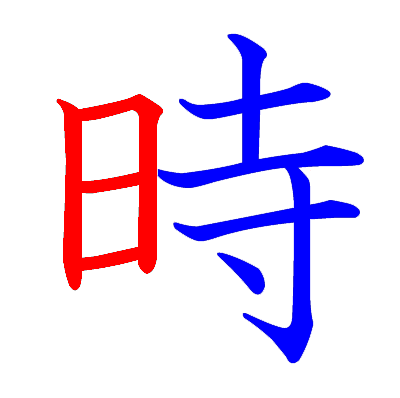
\includegraphics[height=1.2in]{toki-two}
        \caption{Breakdown to simpler Kanji 日\ and 寺}
        \label{fig:toki-b}
    \end{subfigure}
    ~
    \begin{subfigure}[b]{0.3\textwidth}
        \centering
        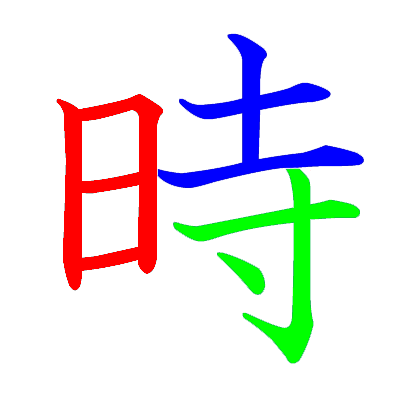
\includegraphics[height=1.2in]{toki-all}
        \caption{Breakdown to the simplest components - radicals 日, 土\ and 寸}
        \label{fig:toki-c}
    \end{subfigure}
    \caption{Breakdown of Kanji 時}
    \label{fig:toki}
\end{figure*}

As with most elements of natural languages, radicals follow Zipf's law. Their distribution can be seen on Figure \ref{fig:zipf}. Frequency axis denotes the number of Kanji featuring each radical. As you can see on the graph, about four fifths of the radicals are featured in less than 50 Kanji. The most common radical appears almost 400 times more often than the least common one.

Some radicals are somewhat similar. It is a concern whether the models will be able to differentiate radical '一' (one) from '二' (two) or a line in '口' (mouth, box). There are many other radicals that look somewhat similar or contain one another in some way. This will be a challenge that may hinder performance of simpler models that don't use convolutions.

\begin{figure*}[h]
    \centering
    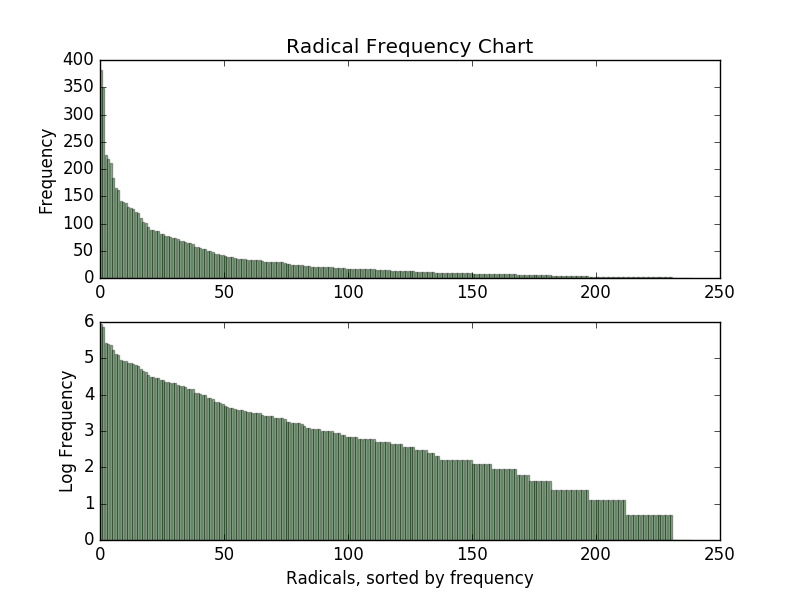
\includegraphics[width=\textwidth]{radicals_zipf}
    \caption{Radical frequency diagram}
    \label{fig:zipf}
\end{figure*}

\section{Related work}
Because Kanji are almost a proper subset of Chinese characters (some characters were modified differently in modern Chinese and Japanese), research into their classification is relevant to this problem. In 2015 Fujitsu has achieved an accuracy rate of 96.7\%, surpassing the human equivalent recognition rate of 96.1\% for classification of Chinese characters\cite{fuji}. A system similar to radical classification was designed in 1982 for on-line Chinese/Kanji character classification by Greanias, E.C. and Yhap, E.F. \cite{greanias1982chinese}. Their system, however, used proprietary set of radicals that they claim can be used to generate all characters. There is a similar stroke-based on-line classifier based on Hidden Markov Models developed by M. Nakai, N. Akira, H. Shimodaira and S. Sagayama that was published by IEEE\cite{953838}. A paper on classification of Japanese scriptures titled "Recognizing Handwritten Japanese Characters Using Deep Convolutional Neural Networks" was published by Charlie Tsai of Stanford University \cite{tsai} that compared classification of all three writing systems using convolutional neural nets of different complexity, ranging from a 6 layer CNN with 4 convolutions to a 16-layer CNN. Tsai reported classification accuracy of 99.64\% achieved on test set by a model that will be explored later in the paper. Tsai's paper mainly focused on classification of Kana scriptures, which he believes is an under-researched field.

\section{Data}
Multiple datasets were used in this project:
\begin{enumerate}
    \item
        Images of handwritten Kanji characters were obtained from the \href{http://etlcdb.db.aist.go.jp/}{Electrotechnical Laboratory (ETL) Character Database}, which has been collected by National Institute of Advanced Industrial Science and Technology (AIST). Specifically, dataset ETL9G was used, which in total contains 421,200 relevant samples. Only 2106 out of 2136 $J\bar{o}y\bar{o}$ Kanji were available because the dataset was collected between '84 and '03, while the missing Kanji were added to the list of $J\bar{o}y\bar{o}$ Kanji in 2010. For each Kanji there are 200 127x128 images provided. \\
        The dataset is stored as 50 files, each file containing 4 images per Kanji.

    \item
        The list of conversion from JIS X 0208 encoding to Unicode characters was obtained from  \href{http://charset.7jp.net/jis0208.html}{charset.7jp.net} - website specialized in collecting tables for different Japanese encodings.
    \item
        Mappings from Kanji to radicals and vice versa were obtained from \href{http://www.Kanjicafe.com/kradfile_license.htm}{RADKFILE and KRADFILE} databases.
    \item
        The list of $J\bar{o}y\bar{o}$ Kanji was obtained from the \href{http://www.bunka.go.jp/kokugo_nihongo/sisaku/joho/joho/kijun/naikaku/pdf/joyoKanjihyo_20101130.pdf}{Agency for Cultural Affairs}, maintained by Japan's Ministry of Education, Culture, Sports, Science and Technology.
\end{enumerate}
Below on Figure \ref{fig:image_samples} are sample images from ETL9G dataset. As you can see, not all samples are perfectly sliced (fig \ref{fig:overlap_sample}) and there might be noise on some samples (fig \ref{fig:noisy_sample}). One's handwriting can really affect the look of the Kanji. An example of that can be shown with Kanji 鋭\ on Figure \ref{fig:handwriting}, on sample \ref{fig:sample-a} the box radical 口\ is distorted so much that it looks like a triangle. The radical below it, 儿\ (legs), is joint in a way that makes it look like another radical, for example 入. Some other examples of this Kanji can be seen on figures \ref{fig:sample-b} and \ref{fig:sample-c}. Again, there are some overlapping characters on these samples.

\begin{figure*}[h]
    \centering
    \begin{subfigure}[t]{0.21\textwidth}
        \fbox{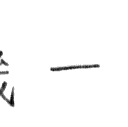
\includegraphics[height=1.2in]{16-76_test}}
        \caption{Overlapping sample}
        \label{fig:overlap_sample}
    \end{subfigure}%
    \begin{subfigure}[t]{0.21\textwidth}
        \fbox{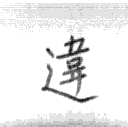
\includegraphics[height=1.2in]{16-67_val}}
        \caption{Sample with noise in the background}
        \label{fig:noisy_sample}
    \end{subfigure}
    \begin{subfigure}[t]{0.21\textwidth}
        \fbox{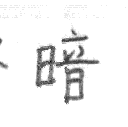
\includegraphics[height=1.2in]{16-37_train}}
        \caption{Sample with noise on the writing}
        \label{fig:noisy_sample2}
    \end{subfigure}
    \caption{Various deformed samples from ETL9G dataset}
    \label{fig:image_samples}
\end{figure*}
\begin{figure}
    \centering
    \begin{subfigure}[t]{0.2\textwidth}
        \fbox{
\includegraphics[height=1.2in]{E98BAD}}
        \caption{Kanji 鋭}
        \label{fig:ideal_sample}
    \end{subfigure}
    \begin{subfigure}[t]{0.2\textwidth}
        \fbox{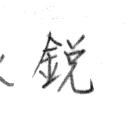
\includegraphics[height=1.2in]{17-52_val}}
        \caption{Messy handwriting}
        \label{fig:sample-a}
    \end{subfigure}
    \begin{subfigure}[t]{0.2\textwidth}
        \fbox{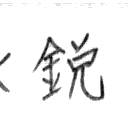
\includegraphics[height=1.2in]{17-52_test}}
        \caption{Example handwriting}
        \label{fig:sample-b}
    \end{subfigure}
    \begin{subfigure}[t]{0.2\textwidth}
        \fbox{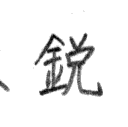
\includegraphics[height=1.2in]{17-52_train}}
        \caption{Example handwriting}
        \label{fig:sample-c}
    \end{subfigure}
    \caption{Different handwriting examples of Kanji 鋭}
    \label{fig:handwriting}
\end{figure}

\section{Methods}
\subsection{Pre-processing}
First, redundant data was removed from all dictionaries, like non-$J\bar{o}y\bar{o}$ Kanji and radicals used only in those Kanji. This resulted in reducing the number of radicals from 252 originally in the dictionaries to 238. Furthermore, some Kanji referenced themselves as their radicals in addition to their actual radicals, but were never used as radicals in any other Kanji. These 3 Kanji (鼓, 香\ and 鼻) were removed from the list of radicals to simplify classification. Using the resulting Kanji-to-radical mapping, all Kanji were encoded using categorical format, where each character is represented by a vector with 1's in the class(es) it belongs to and 0's in the rest. Then the dataset was split into training, validation and testing sets. For direct image-to-Kanji classification 50 or 100 images per Kanji were used to train the models (105300 or 210600 total samples), then 10 images per Kanji were used in each validation and testing sets (21060 samples in each set). For radical classification much smaller sets were needed, because there are less classes and each image belonged to multiple classes. Please see Section \ref{sec:sampling} below for specifics. Testing and validation sets for this model contained 4 images per kanji.

\subsection{Classification}
With each image being 127x128, direct mapping from image to Kanji becomes a very hard problem to train, because the mapping itself is dealing with very large spaces (16256 dimensions to 2106). Classifying Kanji by guessing the radicals is a problem dealing with a much smaller space (16256 dimensions to 235), but a mistake labeling a single radical will result in complete miss-labeling of the input image. Direct classification is the equivalence of classifying a whole English word at once instead of recognizing letters separately: while classifying the whole word is a less ambiguous problem, the search space is much greater than simply classifying the letters.

Four models will be discussed and compared to a baseline set by direct logistic regression:
\begin{enumerate}
    \item A shallow Neural Network with a single hidden layer of 235 layers.
    \item A Neural Network with three fully-connected (FC) hidden layers with 5000 hidden units in each.
    \item A shallow Convolutional Neural Network with four convolutional layers followed by a FC layer with 256 units.
    \item A deeper Convolutional Neural Network with four convolutional layers followed by two FC layers with 4096 hidden units.
\end{enumerate}
The last model is based on the M7-1 model used by Charlie Tsai in his paper: M7-1 was the architecture with best performance on the validation set of Kanji (99.55\%) and second best performance on the test set (99.55\% again, best result was 99.64\%).\\
All convolutional layers feature small 3x3 kernels, number of which differs in each model. Some convolutional layers are followed by max pooling layers with 2x2 kernels. Specific layer breakdown can be seen on table \ref{tab:nets}.\\
REctified Linear Unit (RELU) activation function, defined as $max(0,X)$, was used after each layer.
A version of Model 2 with L2 regularization was also tested, with 0.1 weight coefficient.

\begin{table}[h]
    \centering
    \begin{tabular}{|c|c|c|c|}

    \hline
    Model 1 &Model 2 & Model 3 & Model 4\\[0.5ex]
    \hline\hline
    \multicolumn{4}{|c|}{Input (127x128 Greyscale Image)}\\
    \hline
    &     & conv3 x 32 & conv3 x 64 \\
    &     & conv3 x 32 & \\ \cline{3-4}
    &     & \multicolumn{2}{c|}{maxpool}\\\cline{3-4}
    &     &   conv3 x 64   & conv3 x 128 \\
     &     &   conv3 x 64   &  \\
    \cline{3-4}
    &     &  \multicolumn{2}{c|}{maxpool}\\\cline{3-4}

    &     &      & conv3 x 512 \\
    &     &      & conv3 x 512 \\\cline{4-4}
    &     &      & maxpool\\
    \hline
    FC-235 & FC-5000 & FC-256 & FC-4096\\
           & FC-5000 &         & FC-4096\\
           & FC-5000 &         &\\
    \hline
    \multicolumn{4}{|c|}{FC-Classes}\\
    \hline

    \end{tabular}
    \caption{Neural Net Configurations}
    \label{tab:nets}
\end{table}

\subsection{Sampling}\label{sec:sampling}
Because of Zipfian distribution, using the dataset for training on radicals as-is would overfit on some radicals while still being very untrained on others, since there are Kanji that are radicals of themselves and don't appear anywhere else. To ensure that the models are well trained on the more common radicals, but still know how the less common ones look like, a minimum threshold on the number of the radicals was set. All uncommon radicals are used in conjunction with the most common radicals, so setting a minimum of 200 images per radical ensures that there are enough samples for uncommon ones, but still allows for a possibility of overfitting on the more common ones (there are 11 radicals that appear over 2000 times in a dataset of ~32,000 samples). So, the Zipfian distribution still holds, but the difference is much smaller: before scaling most common radical appeared 400 times more often than the least common, with scaling applied it appears only 20 times more often. The resulting distribution can be seen on the Figure \ref{fig:zipf_scaled} below. Setting the threshold lower keeps the proportion at the same level. Because some radicals are very common, there are many Kanji characters that weren't used to train the model. In fact, only the characters that had unique radicals were included 200 times, other characters had far less samples, many not being needed at all. This allows for a possibility of a radical appearing in a position unseen during training.

\begin{figure*}[h]
    \centering
    \includegraphics[width=\textwidth]{scaled_min=200}
    \caption{Radical frequency after setting minimal threshold to 200 images per radical}
    \label{fig:zipf_scaled}
\end{figure*}

\subsection{Training}

For direct classification softmax was used as the final activation layer with categorical cross entropy as the loss function, defined in equation \ref{eqn:softmax_crossentropy} below:
\begin{multline}\label{eqn:softmax_crossentropy}
    softmax(X) = \frac{e^X}{\sum_{x \in X} e^x}\\
    Cat(X,Y) =  - \sum Y * log(softmax(X))
\end{multline}
For radical classification sigmoid activation layer was used as the input for binary cross entropy, defined in equation \ref{eqn:binary_crossentropy} below. Binary cross entropy was chosen over mean absolute error and mean squared error after training linear regression and Model 2 for 40 epochs with each function.
\begin{multline}\label{eqn:binary_crossentropy}
    sigmoid(X) = \frac{1}{1 + e^{-X}}\\
    Bin(X,Y) = Y * -log(sigmoid(X)) + (1 - Y) * -log(1 - sigmoid(X))
\end{multline}

All models were trained using ADAM optimizer with default parameters described in the paper \cite{DBLP:journals/corr/KingmaB14}.

Learning rate differed depending on the model, ranging from $10^{-4}$ to $10^{-6}$. For example, Model 2 showed no signs of training with learning rate of $10^{-4}$, but simpler models worked perfectly fine. Simpler models converged to the same value using even learning rate of $10^{-3}$, while more complex models required at least $10^{-4}$.

Various batch sizes were tested in different orders of magnitude, from 16 to 15,000. Batches of size 500 have proven to be the most effective, resulting in best performance over 5 epochs.

All models were trained for at least 60 epochs, with simpler models being trained for as many as 400 epochs. An exception to this was Model 4 for direct classification, which was trained for only 24 epochs due to time constraints.

All models were implemented using Keras wrapper for Theano\cite{chollet2015keras}. Training was done on GPU using p2.xlarge instances of Amazon Web Services EC2 servers, except for Model 4, which was trained on CPU using c4.8xlarge instances due to its size. The compiled model was unable to fit on Nvidia Tesla K80 GPU, so training had to be done on CPU.

\subsection{Testing}
\subsubsection{Validation and testing datasets}
While there is a lot of data available in the ETL9G dataset (200 images per character), very little of it was used for validation and testing. For direct classification, validation and testing sets each contained 10 images per Kanji. This amounts to 10\% of the training set each, with the rest of the dataset unused. This kept the sizes manageable while still being enough to gauge the performance. For radical classification less data was used. Because training was done on radicals, but performance is measured on Kanji, no sub-sampling was applied to the testing and validation sets. Instead, each set contained 8 samples of each Kanji, totaling at 16848 samples each. This meant that both training and validation sets each were almost 50\% of the training set in terms of size. On a per-radical basis, however, the relation is very different and varies a lot.

\subsubsection{Accuracy}
For direct classification prediction was considered correct of the maximum value of the softmax layer matched that of the input's one-hot encoding. Then, accuracy was the number of correct predictions over all samples.

For radical classification a similar metric was used. Because by default binary cross entropy is interested in classifying each label separately, its accuracy is not representative of the models actual ability to classify Kanji characters: it could predict that there are no radicals on any image and have accuracy in high 90's. Because of that, accuracy was measured to be the number of samples with each label classified correctly over the total number of samples tested. Specifically, mean absolute error on rounded predictions was used, which is equal to 0 if every label is classified correctly. This metric has also proven to be representative of when a model actually starts learning: some models showed 0\% accuracy for as many as 120 epochs, but when this accuracy started going up, it continued until the model plateaued.

\section{Results and discussion}
Linear regression didn't perform well for neither direct classification nor classification through radicals even after 400 epochs. The former topped with just over 3\% accuracy on the training set and a percent lower on validation and testing. The latter was unable to classify even a single percent of the data, maxing out at 0.024\%. This is a very low baseline for other models to beat.

The rest of the models followed a similar pattern: overfitting everywhere. Other than Models 3 and 4, all models reached reasonably high performance on the training set and a fraction of that on the other sets. Model 2 for direct classification, for example, reached 100\% accuracy on the training set, but on the other sets accuracy was little over 20\%. This model model was also tested with L2 regularization, which showed mixed results. Direct classification was improved by a lot. Even though the model plateaued after 100 epochs, accuracy rose to 72.15\% on validation set and 65.36\% on the training set. Radical classification fell to 0\%, unable to beat the baseline even after 650 epochs. The model was unable to train with different learning rates ($10^{-4}$, $10^{-5}$ and $10^{-6}$ were tested) and smaller batches either. It is possible that such high regularization limited the model's expressiveness, much needed for a target of that complexity.

Model 1 was created to see if it is possible to learn radicals by direct classification, but the model showed poor results and the weights looked like white noise with nightmarish lines imitating Kanji.

Only Convolutional Neural Networks for direct classification had real success. These models were trained on only 50 images per class. Even with such small training set, the small CNN showed 95.57\% classification accuracy on the validation set and 94.43\% on the testing set, which is the closest any of the models has gotten to the human classification rate. With more training it's possible that it would surpass the human recognition rate, the model hasn't converged after 100 epochs and was still showing learning when it had to be terminated. Interestingly, its accuracy on the training set was still very low, barely reaching over 40\%.
When the model was trained again (training data from the previous session was lost), it was unable to reach the same numbers as quickly as before, but the accuracy was still growing steadily after 100 epochs. This newly-trained model achieved 83.44\% on validation set and 78.31\% on the testing set. As before, accuracy on the training set is significantly lower, topping at 35.38\%. Interestingly, the model's performance on validation set grows very fast during the first 50 epochs and slows down during the remaining 50 epochs. On the training set the accuracy grows in a more linear fashion. You can see the whole training history on Figure \ref{fig:history} below.

\begin{figure}[h]
    \centering
    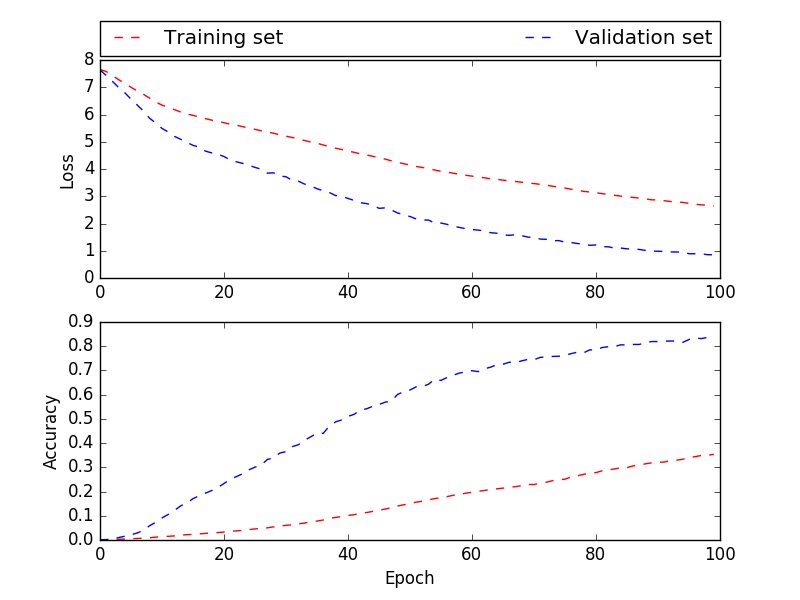
\includegraphics[width=\textwidth]{accuracy_and_loss}
    \caption{Training history of Model 3 with direct targets}
    \label{fig:history}
\end{figure}

The large CNN was showing a lot of promise, but its training had to be aborted due to time constraint. With each epoch taking nearly 2 hours, the net was trained for only 24 epochs and had already achieved an incredible 88.19\% accuracy on validation set. Again, the model showed a lower accuracy (64.69\%) on the training set. Due to implementation semantics, it was impossible to run the testing set through the model and get the accuracy. Still, the model showed consistent increase in accuracy.

The models' radical counterparts, did not perform well at all. Again, this is textbook overfitting: high performance on the training data, low performance on the validation data.

Overall, all models should have been using some sort of regularization and normalization, but overfitting started showing when it was too late to change everything. This was the pitfall for most models, resulting in a gigantic difference between accuracy on the training set and the testing and validation sets. Convolutional networks trumped over regular neural networks and every direct model outperformed its radical counterpart.

Please refer to Table \ref{tab:performance} for accuracy of each model on each set.

\begin{table}[h]
    \centering
    \begin{tabular}{|c|c|c|c|c|c|c|}
        \hline
         & \multicolumn{3}{c|}{Kanji} & \multicolumn{3}{c|}{Radicals}\\
        \cline{2-7}
         & Training & Validation & Test & Training & Validation & Test \\
        \hline
        Baseline & 3.37\% & 2.35\% & 2.56\% & 0.31\% & 0.02\% & 0.02\% \\
        Model 1 & 89.5\% & 19.43\% & 18.74\% & 83.24\% & 0.3\% & 0.3\% \\
        Model 2 & 100\% & 21.13\% & 25.66\% & 80.58\% & 0.39\% & 0.33\% \\
        Model 2 + L2 & 84.69\% & 72.15\% & 65.36\% & 0\% & 0\% & 0\% \\
        Model 3 & 78.94\% & 95.56\% & 94.43\% & 48.77\% & 2.69\% & 3.27\% \\
        Model 4 & 64.69\% & 88.19\% & N/A & 90.38\% & 33.71\% & 37.64\% \\
        \hline
    \end{tabular}
    \caption{Classification accuracy of all models}
    \label{tab:performance}
\end{table}

\section{Conclusion}
In this paper we have explored a viability of classification of Japanese Kanji characters via radicals, their building blocks. While the unique mapping exists and theoretically classifying radicals is a more sensible approach, none of the models tested were able to classify radicals accurately enough to achieve level close to that of their direct classification counterparts, let alone human classification rate. Most models tested showed signs of overfitting the training data. Attempts to reduce its effects showed mixed results by boosting performance of direct model and completely nullifying performance of radical classification.

Earlier an analogy was made about classifying Kanji as classifying complete English words. This paper showed that despite this being a less elegant solution to the problem, 2106 unambiguous characters is still doable even with a simple Convolutional Neural Network. Less complex models were unable to show anything interesting and more complex models take a lot of time to train even with a smaller training dataset. One advantage radical classification has over direct classification is complexity of the mapping. With almost 10 times less classes, each training step took fraction of time used for direct classification. The best example of this is Model 2. Both direct and radical classifications started training at the same time on same configurations, both trained on GPU with the same parameters. By the time the direct model completed its 150th epoch, radical classification was already over 600 epochs in. Unfortunately, that particular model did not show good results, but this is still a good example of how much harder it is to train a complex function with 10 times more classes.

There is still room for more research on this subject. One direction for improvement is restricting the number of radicals to the official set of 214 Kangxi radicals or a custom set of characters like Greanias, E.C. and Yhap, E.F. have done for their model. There is also room for improvement with model architecture. Model 3 has shown that even small models can achieve high classification rate. Building models more tailored for this problem can improve performance. Using binarized dataset can simplify learning and classification. It was too late to add regularization to these models and properly test them, but there is definitely room for improvement in that direction as well.


\bibliography{references}{}
\bibliographystyle{plain}

\end{CJK*}
\end{document}


%\begin{figure}
%    \centering
%    \includegraphics{weights}
%    \caption{Weights of the net from A2}
%    \label{fig:weights}
%\end{figure}
